\documentclass{protokol}

\usepackage[czech]{babel}
\usepackage[utf8]{inputenc}
\usepackage{icomma}

% Plovouci bloky (obrazky, tabulky)
\usepackage{floatrow}
\floatsetup[table]{capposition=top}
\floatsetup[figure]{frameset={\fboxsep16pt}}
\usepackage{subcaption}

% Tabulky
\usepackage{tabu}
\usepackage{booktabs}
\usepackage{csvsimple}
\usepackage{multirow}
\usepackage{multicol}

% Jednotky
\usepackage{siunitx}
\sisetup{
	locale               = DE,
	inter-unit-product   = \ensuremath{{}\cdot{}},
	list-units           = single,
	list-separator       = {; },
	list-final-separator = \text{ a },
	list-pair-separator  = \text{ a },
	range-phrase         = \text{ až },
	range-units          = single,
}
\usepackage{amsmath}

% Obvody
\usepackage{circuitikz}

% Obrazky a grafy
% \usepackage{graphicx}
\graphicspath{
	{img/}
	{plots/}
	{build/plots/}
}
\usepackage{epstopdf}
\epstopdfsetup{outdir=./build/plots/}

\usepackage[hidelinks,pdfusetitle]{hyperref}
\usepackage[backend=biber, sorting=none, sortlocale=cs_CZ]{biblatex}
\addbibresource{references.bib}

\title{Langmuirova sonda}
\author{Pavel Kosík, Jan Slaný}

\jmenopraktika={Praktikum z fyziky plazmatu}  % jmeno predmetu
\jmeno={Pavel Kosík, Jan Slaný}                             % jmeno mericiho
\obor={F}                               % zkratka studovaneho oboru
\skupina={Út 15:00}                     % doba vyuky seminarni skupiny
\rocnik={IV}
\semestr={VIII}

\cisloulohy={03}
\jmenoulohy={Langmuirova sonda}

\datum={8. března 2022}                  % datum mereni ulohy
\tlak={}% [hPa]
\teplota={}% [C]
\vlhkost={}% [%]

\newcommand\elemcharge{e}
\newcommand\boltzmann{k}
% \newcommand\boltzmann{k_\mathrm{B}}
\newcommand\masselec{m_\mathrm{e}}

\newcommand\pres{p}
\newcommand\idisch{I_\mathrm{d}}
\newcommand\iprobe{I_\mathrm{s}}
\newcommand\iion{I_\mathrm{i}}
\newcommand\ielec{I_\mathrm{e}}
\newcommand\flpot{V_\mathrm{fl}}
\newcommand\plpot{V_\mathrm{p}}
\newcommand\potprobe{V_\mathrm{s}}
\newcommand\uprobe{U_\mathrm{s}}
\newcommand\dension{n_\mathrm{i}}
\newcommand\denselec{n_\mathrm{e}}

\begin{document}
\header

\newcommand\parta{A}
\newcommand\partb{B}
\newcommand\partc{C}
\newcommand\probesurf{S}
\newcommand\tempelec{T_\mathrm{e}}
\section{Úvod}
V~této úloze se budeme zabývat studiem kladného sloupce doutnavého výboje
pomocí Langmuirovy sondy.
Výstupem bude koncentrace elektronů a jejich teplota.
Langmuirovou sondou rozumíme vodič s malými rozměry zavedený do~plazmatu.
Potenciál sondy označme jako~$\potprobe$ a proud protékající sondou
jako~$\iprobe$.
Základní princip měření spočívá v~určení závislosti proudu~$\iprobe$
protékajícího sondou na potenciálu sondy~$\potprobe$.
Analýzou této voltampérové charakteristiky lze učit některé parametry plazmatu.

Langmuirova sonda svou přítomností ovlivňuje zkoumané plazma,
proto je vhodné, aby byla co nejmenší.

\subsection{Jednoduchá sonda}
Jednoduchá Langmuirova sonda sestává z~jediného vodiče vnořeného do plazmatu.
Typická voltampérová chrakteristika rovinné sondy je na~obrázku
č.~\ref{fig:vac-simple} a~její průběh můžeme rozdělit na tři oblasti.

\begin{figure}[hbp]
	\centering
	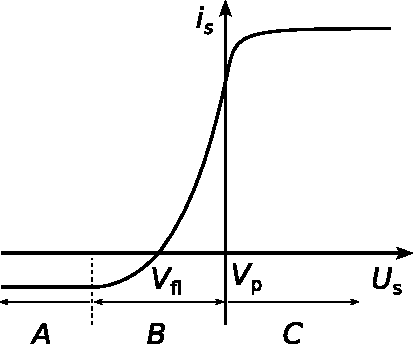
\includegraphics{vac-simple}
	\caption{Voltampérová charakteristika jednoduché sondy.
		Převzato z~\autocite{assignment-simpleprobe}.}
	\label{fig:vac-simple}
\end{figure}

\subsubsection{Oblast saturovaného proudu \parta}
Pokud je sonda výrazně záporně nabitá vzhledem k potenciálu plazmatu,
uplatní se Debyeovo stínění a~v~okolí sondy vznikne vrstva kladného
prostorového náboje.
Jelikož v této vrstvě nejsou elektrony, nemůže zde probíhat rekombinace,
ionizace, ani excitace nárazem elektronu a kolem sondy pozorujeme temný prostor.
Proud dopadající na sondu je převážně iontový
a~jeho velikost se řídí Child-Langmuirovým zákonem.

\subsubsection{Přechodová oblast \partb}
Při zvýšení napětí na sondě získají některé elektrony dostatečnou energii na to,
aby překonaly stěnovou vrstvu a dopadly na povrch sondy.
Iontový proud stále převládá.
Absolutní hodnota proudu s~rostoucím napětím na sondě klesá.
Bod, pro nějž je roven nule (tedy tam, kde se proudové příspěvky vyrovnají)
se nazývá plovoucí potenciál $\flpot$.
Další zvyšování napětí na sondě $\potprobe$ má za následek růst celkového proudu.
Zde již převládá proud elektronový $\ielec$, jehož průběh v~této oblasti lze
za předpokladu Maxwell-Boltzmannova rozdělení popsat vztahem:
\begin{equation}
	\ielec = \probesurf \elemcharge \denselec
		\sqrt{\frac{\boltzmann \tempelec}{2 \pi \masselec}}
		e^{\frac{-\elemcharge\uprobe}{\boltzmann \tempelec}},
\end{equation}
jde $\probesurf$ je plocha sondy, $\denselec$ koncentrace elektronů,
$\boltzmann$ Boltzmanova konstanta a~$\elemcharge$ náboj elektronu.
Nastává změna polarizace sondy.
Závislost $\ln(\ielec)=f(\uprobe)$ by měla být lineární.
Směrnice přímky potom určuje teplotu elektronů $\tempelec$
a~konstantní člen koncentraci elektronů $\denselec$.

\subsubsection{Oblast saturovaného elektronového proudu \partc}
Je-li překročeno nulové napětí $\uprobe$ na sondě
(tedy je-li sonda nabita vzhledem k potenciálu plazmatu $\plpot$ kladně),
začíná sonda přitahovat elektrony a odpuzovat kladné ionty.

V~případě válcové sondy proud v~této oblasti parabolicky roste.

\section{Metoda}
Byla použita sonda s válcovou geometrií
o~poloměru $r=\SI{0.1}{\milli\metre}$ a délce $l=\SI{8}{\milli\metre}$.

\section{Výsledky}
Naměřené voltampérové charakteristiky jsou na obrázcích
č.~\ref{fig:vac-1}--\ref{fig:vac-6}.

\newcommand\figvac[3]{
	\begin{figure}[htp]
		\centering
		\input{plots/vac-#1}
		\input{plots/vac-log-#1}
		\caption{Voltampérová charakteristika sondy
			při výbojovém proudu $\idisch = \SI{#2}{\milli\ampere}$
			a tlaku $\pres = \SI{#3}{\pascal}$.}
		\label{fig:vac-#1}
	\end{figure}
}

\figvac{1}{50}{50}
\figvac{2}{40}{50}
\figvac{3}{30}{50}

\figvac{7}{50}{100}
\figvac{4}{50}{20}
\figvac{5}{50}{10}
\figvac{6}{50}{5}

\printbibliography
\end{document}
